%%%%%%%%%%%%%%%%%%%%%%%%%%%%%%%%%%%%%%%%%%%%%%%%%%%%%%%%%%%%%%%%%%%%%%%%
%                                                                      %
%     File: Thesis_Static_Features.tex                                 %
%     Tex Master: Thesis.tex                                           %
%                                                                      %
%     Author: João C. Godinho                                          %
%     Last modified : Apr 2018                                         %
%                                                                      %
%%%%%%%%%%%%%%%%%%%%%%%%%%%%%%%%%%%%%%%%%%%%%%%%%%%%%%%%%%%%%%%%%%%%%%%%

\chapter{Static Features}
\label{chapter:static_features}

In the present chapter we go into details about how we built a machine learning model to detect malware based on static features.
We start by detailing the model selection and its evaluation, followed by the selected features.
We finish off by providing how our model performed under various scenarios.

%%%%%%%%%%%%%%%%%%%%%%%%%%%%%%%%%%%%%%%%%%%%%%%%%%%%%%%%%%%%%%%%%%%%%%%%
\section{Model Selection and Evaluation}
\label{section:model_selection_evaluation}

In this section we go over the classifier used to create the model that separates malware from goodware, as well as our evaluation methodology.

%%%%%%%%%%%%%%%%%%%%%%%%%%%%%%%%%%%%%%%%%%%%%%%%%%%%%%%%%%%%%%%%%%%%%%%%
\subsection{Model Selection}
\label{section:model_selection}

Our main concerns when choosing a classifier regard the ability to produce a probabilistic output (\ie\ probability of being malware), good scaling for large number of features and samples and ease of use.

Taking into consideration the guidelines given in~\cite{rossow:practices,shabtai:survey} and related work in~\cite{miller:rev_int,nissim:al_pdf,rieck:dynamic,schultz:data_mining}, we decide to use \textit{\acrfull{lr}} as our model.
This model fits our needs as it gives the probability of a random variable $X$ being 0 or 1, given a set of constraints (\ie~features), scales well with samples and features and it is readily available from several libraries, facilitating implementation~\cite{friedman2001elements}.

\gls{lr} can be defined with the form
\begin{eqnarray*}
	\rho(x) = \dfrac{1}{1 + e^{-x}},&x = \beta_0 + \beta_1x_1 + ... + \beta_nx_n
\end{eqnarray*}
where $\beta_n$ is the learned weight for feature $x_n$.
This weight is learned through iteration in order to minimize the error between the predicted values and the actual values.
In other words, given an \textit{n-th} dimensional set of features, \gls{lr} will try to create an hyperplane that divides samples from two classes.

As \gls{lr} is based on the logistic function (or sigmoid function, visually represented in Figure \ref{fig:sigmoid_function}), each feature $x_n$ can vary from $-\infty$ to $+\infty$ and still the output is contained between 0 and 1, hence providing probabilistic values.

\begin{figure}[!h]
	\centering
	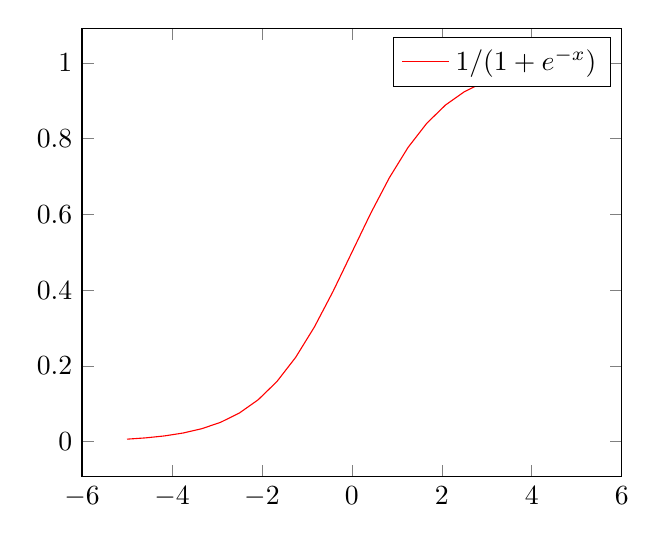
\begin{tikzpicture}
	\begin{axis}
	\addplot[
		color=red,
		domain=-5:5
	]
	{1/(1+exp(-x))};
	\addlegendentry{$1/(1+e^{-x})$}
	\end{axis}
	\end{tikzpicture}
	\caption{Sigmoid function $f(x)=\dfrac{1}{1+e^{-x}}$}
	\label{fig:sigmoid_function}
\end{figure}

To implement this model we take advantage of scikit-learn~\cite{tool:sklearn} library, a Python library that provides a multitude of models and tools that facilitate the creation of \gls{ml} models.

%%%%%%%%%%%%%%%%%%%%%%%%%%%%%%%%%%%%%%%%%%%%%%%%%%%%%%%%%%%%%%%%%%%%%%%%
\subsection{Evaluation}
\label{section:evaluation}

With regards to our evaluation methodology, as we have previously mentioned, our purpose is to understand how laboratory conditions compare to real-world conditions.
We now detail how we achieve and compare these conditions.

Given the purpose of our work, we choose to measure our results by plotting an \gls{auroc} graph, which measures the \tpr~at different \fpr~levels, metrics that are commonly used across similar work~\cite{miller:rev_int,nissim:al_pdf,schultz:data_mining}.

Our first evaluation methodology is to apply a common \gls{ml} validation technique named \textit{k-fold cross-validation}, with $k=10$, depicted in Figure \ref{fig:xval}.
This method works by splitting the dataset into $k$ equally sized parts (folds) and then trains using $k-1$ folds, using the remaining fold as validation.
This process is repeated $k$ times, guaranteeing that every fold is used at least once for validation.
This methodology is useful to prevent over-fitting, as the validation fold is never used together with the training folds.

\begin{figure}[!htb]
	\centering
	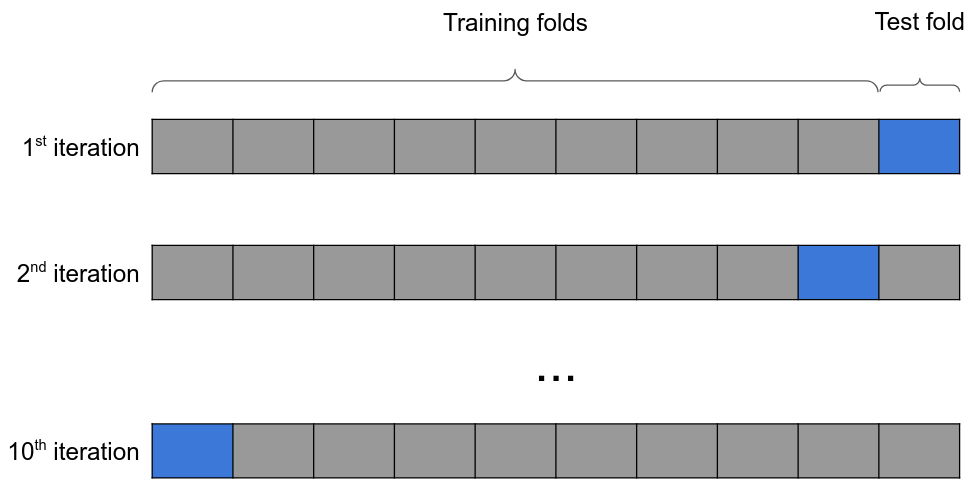
\includegraphics[width=0.8\textwidth]{Figures/dia_xvalidation.png}
	\caption[Cross-validation evaluation example.]{Cross-validation evaluation example with $k=10$ folds.}
	\label{fig:xval}
\end{figure}

This evaluation methodology is our baseline, hence we define it as our \textit{laboratory} conditions, where no time based consistency is taken into account.

\medskip

Although the cross-validation methodology enables to measure the generalization capabilities of a model, it does not account for temporal ordering of the samples.
Since we want to measure the when training samples predate validation, we now define a couple of temporal based validations, based on the concept of cross-validation:

\paragraph{\textit{Past-to-Present}:} This validation, depicted in Figure \ref{fig:past_present}, can be resumed as an iterative methodology where the validation set is a fixed percentage of dataset's most recent samples, whereas the training set is a fixed percentage of the dataset's oldest.
The training set is split into $k$ temporal consistent folds and at each iteration it is extended with more recent folds and scored against the training set, until all folds are used.

\begin{figure}[!htb]
	\centering
	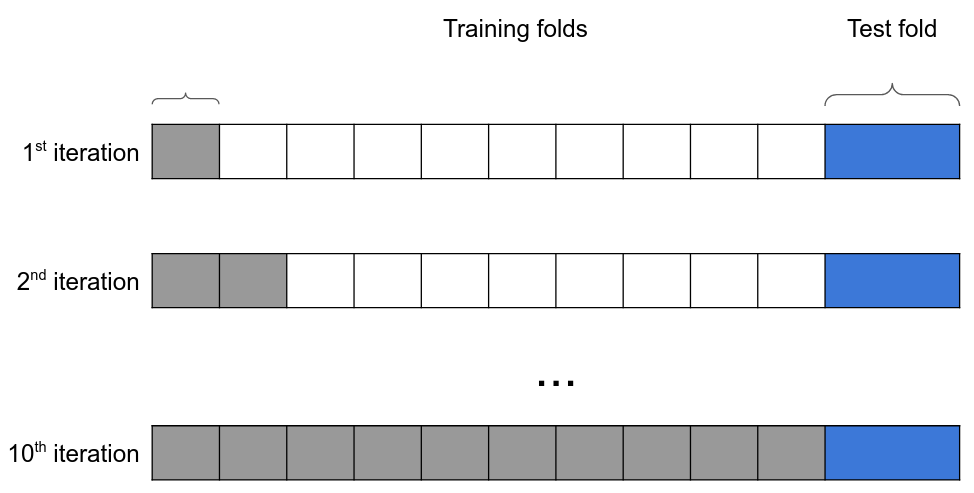
\includegraphics[width=0.8\textwidth]{Figures/dia_pastpresent.png}
	\caption[Past-to-Present evaluation example.]{Past-to-Present evaluation example with 20\% test, 80\% training, $k=10$ folds in training.}
	\label{fig:past_present}
\end{figure}

\paragraph{\textit{Present-to-Past}:} This validation, depicted in Figure \ref{fig:present_past}, is the opposite of \textit{Past-to-Present} with regards to the starting point of the training set.
Again the validation is fixed at the most recent samples, but the training set starts with the temporally closest fold to the validation set.
At each iteration the training set is extended, this time with older folds, and scored against the validation, until all folds are used.

\begin{figure}[!htb]
	\centering
	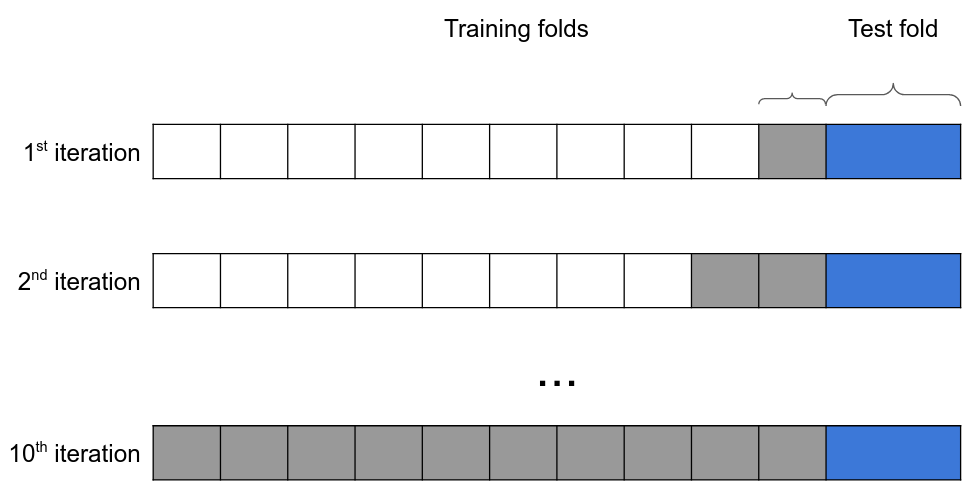
\includegraphics[width=0.8\textwidth]{Figures/dia_presentpast.png}
	\caption[Present-to-Past evaluation example.]{Present-to-Past evaluation example with 20\% test, 80\% training, $k=10$ folds in training.}
	\label{fig:present_past}
\end{figure}

\medskip
Both \textit{Past-to-Present} and \textit{Present-to-Past} validations require two parameters: the size of the validation set and how the increments to the training set are made.
For the purpose of our work, we use the 20\% most recent samples for validation, and split the remaining 80\% into 10 folds, hence the validation is done 10 times, with each iteration increasing the training set size by one fold.

These two validation methodologies give us the ability to account for temporal consistency.
Moreover, they enable us to compare the importance of older \textit{vs.}\ newer samples to classify recent samples.

\paragraph{\textit{Temporal Window}:} This validation, depicted in Figure \ref{fig:sliding_window}, also splits the dataset into $k$ folds, but takes $w$ temporal consistent and contiguous folds (\ie each fold immediately precedes the next one), using the first $w-1$ folds for training (older samples) and the remaining fold (more recent samples) for validation.
By starting with the $w$ first folds of the dataset and sliding one fold on each iteration, we apply a sliding window of size $w$ over the dataset.
For this last validation methodology, we again split the dataset into 10 folds.
The sliding window size $w$, is chosen during the results phase, as its choice depends on previous results.

\begin{figure}[!htb]
	\centering
	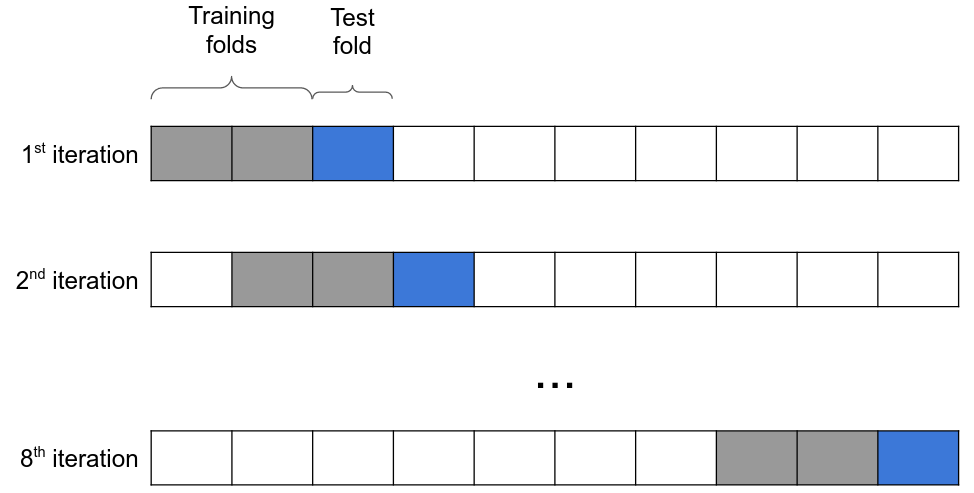
\includegraphics[width=0.8\textwidth]{Figures/dia_slidingwindow.png}
	\caption[\textit{Temporal Window} evaluation example.]{\textit{Temporal Window} evaluation example with $w=3$ window size over $k=10$ folds.}
	\label{fig:sliding_window}
\end{figure}

\medskip

As we have previously described in Section \ref{section:dataset_creation}, we possess 3 different datasets, created from 3 different scenarios.
With that in mind, all our previously described methodologies: cross-validation, past-to-present and present-to-past; are applied to each of the 3 datasets.

Applying the aforementioned methodologies to our 3 datasets enables us to study not only how temporal consistency impacts the results, but also the impact of \textit{ground-truth}.

%%%%%%%%%%%%%%%%%%%%%%%%%%%%%%%%%%%%%%%%%%%%%%%%%%%%%%%%%%%%%%%%%%%%%%%%
\section{Feature Selection}
\label{section:feature_selection}

One of the most important stages in Machine Learning is the selection of the features to analyze, and features based on static imports have shown promising results in \gls{ml} applications for malware detection~\cite{miller:rev_int,schultz:data_mining}.
In this section we describe the adopted static features that were fed into our model.

Although Cuckoo provides enormous amounts of usable information, we chose to start with simple features as to have a basic understanding of how doable our approach is.
More so, one of our main concerns is how the same feature gives different results under our different scenarios, hence the performance between scenarios and methodologies is more relevant than absolute performance.
With that in mind, we chose to use the static imports as features.

Static imports are present in the import table, referencing libraries or other executables that are not part of the current binary.
Their usage is key, as they provide access to all kind of system level operations (\eg\ file manipulation, network access). Given their purpose, our expectation is that a sample's maliciousness can be inferred based on the static imports.

Using Celery~\cite{tool:celery}, a distributed task queue for Python, we optimized the parsing of the available HTML reports, extracting samples that contained information regarding static imports into a new set $\DD_{static}$.
We then joined the samples with static imports $\FF_{static}$ to the labeled samples $\CC_{real}$, obtaining a total of 189,352 labeled samples with static imports $\DD_{static} = \CC_{real} \cap \FF_{static}$.

We then vectorized imports by creating a binary vector where each position corresponds to a specific import.
If a given import $i$ is present in a sample, its feature vector $x$ will have the value 1 at that position $x_i$.
Likewise, if a given import $j$ is not present in a sample, its feature vector $x$ will have the value 0 at that position $x_j$.

Due to the amount of samples and variety of imports, each sample got a vector $x$ of 6,647 dimensions (\ie\ there are 6,647 different imports).
To reduce this number, and to remove any noise due to incorrect parsing of static imports by Cuckoo, we applied a variance threshold.

The variance threshold calculates the variance for each import, removing those that are below a given threshold.
In our case, since we are working with a binary vector, each import can be represented as Bernoulli random variable, hence their variance is given by $p(1-p)$.
With that in mind, we removed any import that did not vary in more than 99\% of samples.

The resulting dataset $\FF_{static}$ got reduced to 187,545 samples, each with a 64 dimensional binary vector.

%%%%%%%%%%%%%%%%%%%%%%%%%%%%%%%%%%%%%%%%%%%%%%%%%%%%%%%%%%%%%%%%%%%%%%%%
\section{Single Layer Results}
\label{section:single_layer_results}

Having met all the necessary conditions to build a \gls{ml} model: model selection and evaluation and feature selection, we are now ready to provide the results of our first experiments.

Using an Ubuntu Virtual Machine with 16 cores and 16GB of RAM, provided by INOV - Inesc Inovação, and taking advantage of scikit-learn~\cite{tool:sklearn} to train the models, Pandas~\cite{tool:pandas} for data analysis and Jupyter Interactive Notebooks~\cite{tool:jupyter} to interact with the Python scripts, we now detail our logistic regression model results.

We define this our single layer model $\LR$ results, as we are directly taking a set of features (static imports in this case) and outputting the probability of a sample being malware.

\medskip
%%%%%%%%%%%%%%%%%%%%%%%%%%%%%%%%%%%%%%%%%%%%%%%%%%%%%%%%%%%%%%%%%%%%%%%%
% \subsection{Laboratory Conditions}
% \label{section:single_layer_laboratory}

We start with what we define as \textit{laboratory conditions}, ideal conditions for the problem of malware detection.
These conditions are met when we take the labeled dataset $\CC_{strict}$ and features $\DD_{static}$, providing scenario $\mathcal{S}_{\strict}$.

Using cross-validation, our $\LR$ scored with an \gls{auroc} of \miss{score}, as shown by the red line in Figure \ref{fig:xval_results}.
We argue that such high values are easily attained from factors like a small and reliable dataset, and the use of cross-validation, which mixes samples and ignores possible dependencies on malware samples.

When we relax our ideal conditions to more \textit{real-world conditions}, by testing the labeled dataset $\CC_{loose}$ and $\CC_{real}$ on features $\DD_{static}$ for scenarios $\mathcal{S}_{loose}$ and $\mathcal{S}_{real}$, respectively, the score under \gls{auroc} decreases to \miss{score} for $\mathcal{S}_{loose}$ (blue line in Figure \ref{fig:xval_results}) and \miss{score} for $\mathcal{S}_{real}$ (green line in Figure \ref{fig:xval_results}).

\begin{figure}[!htb]
	\centering
	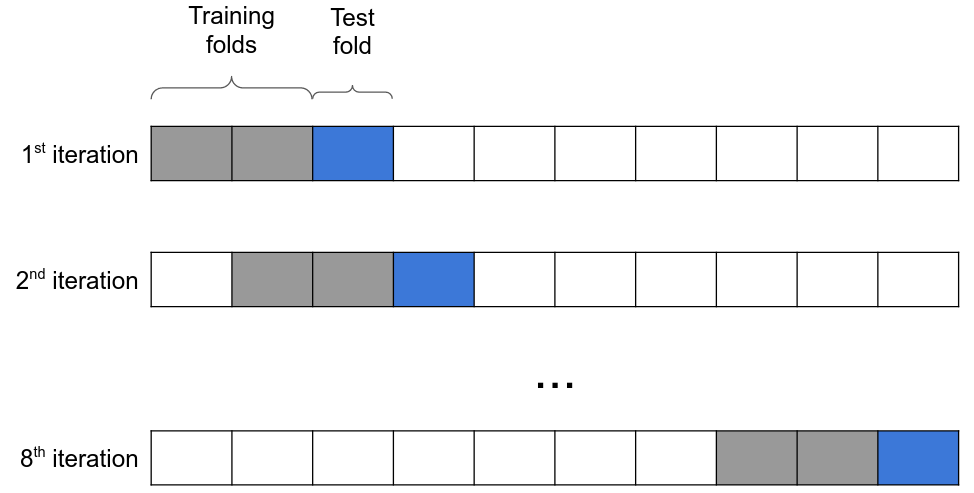
\includegraphics[width=0.8\textwidth]{Figures/dia_slidingwindow.png}
	\caption[Single layer results for static features in laboratory conditions.]{Single layer results for static features in laboratory conditions.}
	\label{fig:xval_results}
\end{figure}

From $\mathcal{S}_{\strict}$ to $\mathcal{S}_{\loose}$, the only change is the amount of malware labeled samples, which significantly increase.
The difference is interesting, as although the number of malware labeled samples increase significantly, the results are not that affected.
This suggests that although the reliability for malware decreases, its impact is not as noticeable as expected.
This might also suggest that vendors do converge on their definition of malware, under our $\Mloosev$ metric.
If vendors did not converge on what is malware, adding more samples would culminate in worse results, as separation between malware and goodware would become harder.

When looking at the changes from $\mathcal{S}_{\loose}$ to $\mathcal{S}_{\real}$, not only the amount of malware labeled samples increase, but also the number of goodware labeled samples, both by a significant amount. 
The way this impacts the results is pretty significant, as we observe a high decrease in the \gls{auroc} for both models.
The metric $\Mrealv$ that labels malware and goodware for this scenario $\mathcal{S}_{\real}$ disregards the cross-check from outside repositories, which in turn degrade the reliability significantly, as well as increase the dataset size notably.
We attribute the results' degradation mainly to the unreliability of goodware labeling, not only because we have previously seen that increase in malware does not significantly impact results (from $\mathcal{S}_{\strict}$ to $\mathcal{S}_{\loose}$), but also due to the tendency for false negatives in vendors (Figure \ref{fig:dups_frequency}), which in turn lead us to incorrectly label goodware for the samples in $\CC_{real}$.

The results we described show how relaxing \textit{laboratory conditions} to more \textit{real-world conditions} degrade the model's performance.
We now focus on using our previously defined temporal based methodologies to further converge into a real-world scenario.

\medskip

We start by applying our \textit{Past-to-Present} validation to the three scenarios, $\mathcal{S}_{\strict}$, $\mathcal{S}_{\loose}$ and $\mathcal{S}_{\real}$.
As previously defined, this validation starts with an older set of training samples and iteratively adds newer samples, validating each iteration on a fixed set of the most recent samples.
Since our interest is to measure performance variation over time, we plot in Figure~\ref{fig:pastpresent} the \gls{auroc} at every iteration (\ie, fold), for each of our three scenarios.

\begin{figure}[!htb]
	\centering
	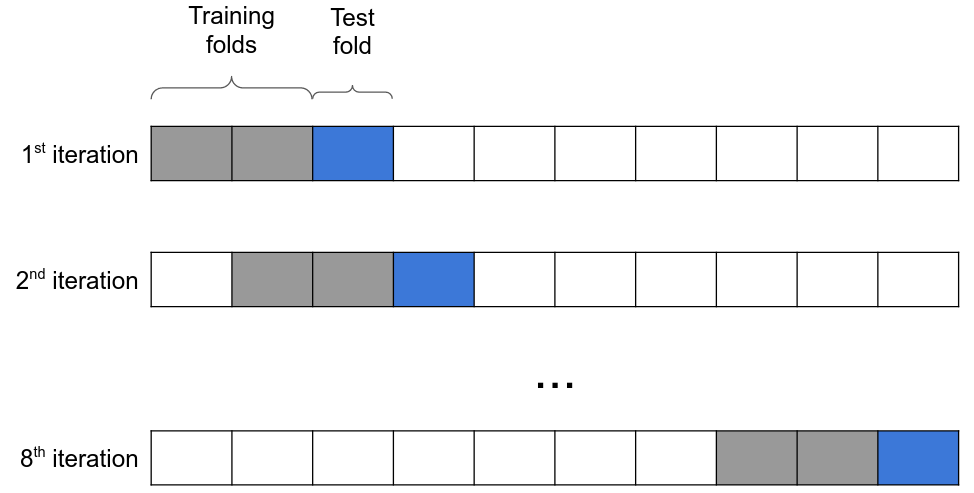
\includegraphics[width=0.8\textwidth]{Figures/dia_slidingwindow.png}
	\caption[Single layer results for static features in \textit{Past-to-Present}.]{\gls{auroc} for each iteration of the \textit{Past-to-Present} evaluation. Folds order consistent with temporal order (\ie\ fold 0 contains older samples than
fold 1)}
	\label{fig:pastpresent}
\end{figure}

When directly comparing the average \gls{auroc} for cross-validation and our \textit{Past-to-Present} validation, we note a decrease from \miss{score} to \miss{score} for $\mathcal{S}_{\strict}$, \miss{score} to \miss{score} for $\mathcal{S}_{\loose}$, and \miss{score} to \miss{score} for $\mathcal{S}_{\real}$.
This decrease is intuitive to the methodology, as we are forcing temporal consistency between samples.

When looking at results from $\mathcal{S}_{\strict}$ and $\mathcal{S}_{\loose}$, we see they closely relate.
This relation has already been noticed on previous cross-validation results, as their metrics $\Mstrictv$ and $\Mloosev$ are not very different.
As for $\mathcal{S}_{\real}$, the degradation is higher, as the reliability of the metric $\Mrealv$ goes down.

Our main observation for this validation methodology is that there is a slight tendency for \gls{auroc} to increase, as we move forward in time, close to the validation set.

Both $\mathcal{S}_{\strict}$ and $\mathcal{S}_{\loose}$ behave similarly under our \textit{Past-to-Present} evaluation, decreasing the \gls{auroc} until fold \miss{fold}, after which both increase, stabilizing around \miss{score} \gls{auroc} by the last \miss{two} folds. As for $\mathcal{S}_{\real}$, its \gls{auroc} does not vary significantly, although a subtle increase over time is noticeable.

\medskip

Our next result, which uses our \textit{Present-to-Past} validation methodology will further help analyze the aforementioned detail.
The \textit{Present-to-Past} validation enhances the previous results under real-world conditions.
This methodology starts by fixing the validation set to the most recent samples, but with the training set starting at the temporally closest samples to validation.
At each iteration, older samples are added to the training set and validated on the fixed, most recent, samples.

By applying this methodology to the three scenarios, $\mathcal{S}_{\strict}$, $\mathcal{S}_{\loose}$ and $\mathcal{S}_{\real}$, we plot Figure \ref{fig:presentpast}, where the X axis increases as older samples are added to the training set (\ie\ fold 0 contains newer samples than fold 1), hence measuring the performance variance over time.
Similarly to the previous observation, the average \gls{auroc} suffers a decrease when compared to cross-validation. For $\mathcal{S}_{\strict}$ we note a change from \miss{score} to \miss{score}, for $\mathcal{S}_{\loose}$ the decrease is from \miss{score} to \miss{score}, and for $\mathcal{S}_{\real}$ \miss{score} to \miss{score}.

\begin{figure}[!h]
	\centering
	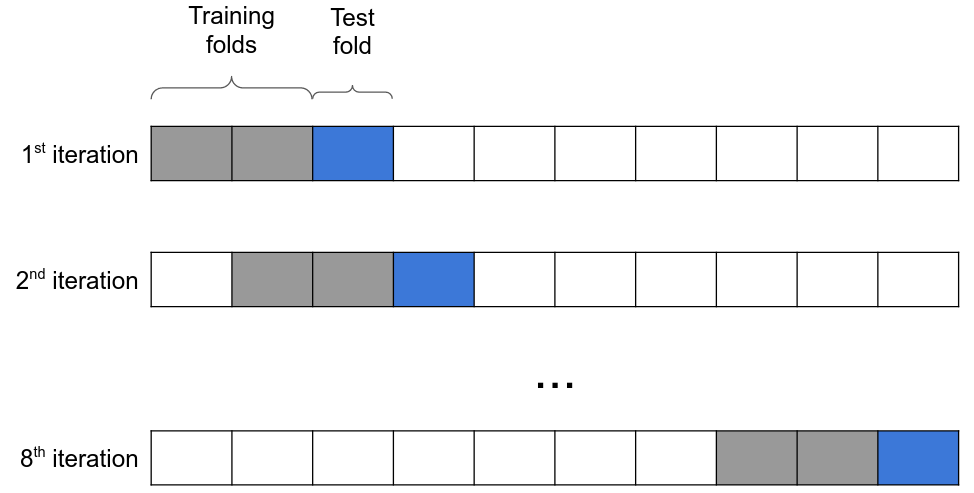
\includegraphics[width=0.8\textwidth]{Figures/dia_slidingwindow.png}
	\caption[Single layer results for static features in \textit{Present-to-Past}.]{\gls{auroc} for each iteration of the \textit{Present-to-Past} evaluation. Folds order is the inverse of temporal order (\ie\ fold 0 contains newer samples than fold 1)}
	\label{fig:presentpast}
\end{figure}

The comparison between scenarios is identical to what was observed in cross-validation and \textit{Past-to-Present}: scenarios $\mathcal{S}_{\strict}$ and $\mathcal{S}_{\loose}$ display very similar results, with $\mathcal{S}_{\real}$ dropping behind due to its less reliable labeling metric.

With these results, our original observation that samples closer to the validation set benefit the model becomes more convincing. In fact, we argue that there should be an ideal number of necessary training folds, temporally consistent with the validation fold (\ie\ any fold from training predates validation), needed to maximize the overall score.

\medskip

Finally, we analyze how does such reduced training set behaves in our scenarios; for this purpose, we define a sliding window that moves forward in time through each scenario for training and validation.
We propose a reduction on the training size to \miss{$w=3$} folds predating the validation fold. We choose \miss{$w = 3$}, since we have seen that the scores either do not improve (for $\mathcal{S}_{\strict}$ and $\mathcal{S}_{\loose}$) or actually go down (for $\mathcal{S}_{\real}$) with higher folds.
In summary, we have selected \miss{30\%} of each dataset for training purposes and the next \miss{10\%} for validation \miss{(3 training folds, 1 validation fold)}, and then started moving the window forward in time (1 fold at a time) to obtain the following results (Figure~\ref{fig:slidingwindow}): for  $\mathcal{S}_{\strict}$, $\mathcal{S}_{\loose}$ and $\mathcal{S}_{\real}$, we obtain \gls{auroc} values of \miss{score, score and score}, respectively. 
These results come to reaffirm our argument that we can reduce the size of the training set, without losing any significant score.

\begin{figure}[!h]
	\centering
	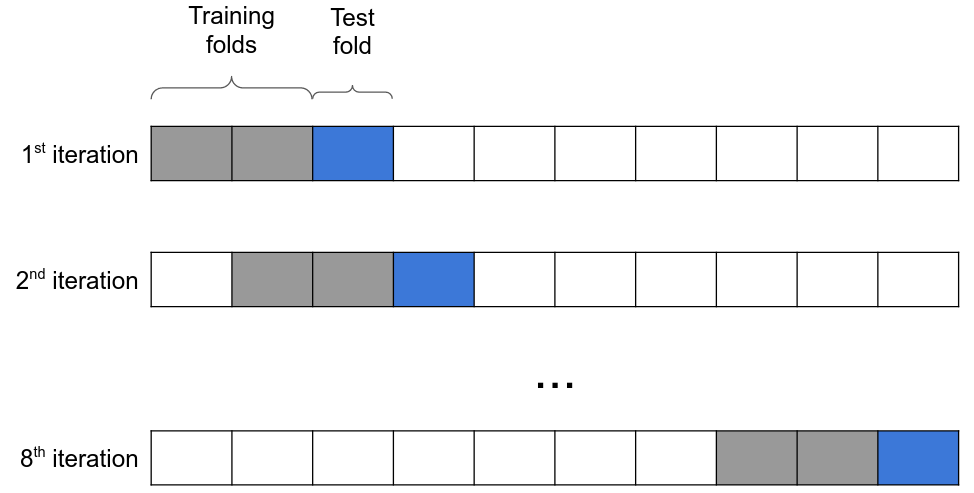
\includegraphics[width=0.8\textwidth]{Figures/dia_slidingwindow.png}
	\caption[Single layer results for static features in \textit{Temporal Window}.]{\gls{auroc} for our three scenarios, under the \textit{Temporal Window} methodology.}
	\label{fig:slidingwindow}
\end{figure}

Comparing these results with the baseline cross-validation, we note a decrease for each scenario, specifically a decrease from \miss{0.93 to 0.87 for $\mathcal{S}_{\strict}$, from 0.92 to 0.86 for $\mathcal{S}_{\loose}$ and from 0.79 to 0.76 for $\mathcal{S}_{\real}$.}
We should highlight that the results that use temporal-consistency should better reflect the reality than standard cross-validation, since we are requiring temporal consistency.
Another important idea that should be stressed is that for cross validation we used a fairly reasonable amount of data for training purposes, whereas in this last case we used a restricted amount of data. This might be a relevant issue in a few year's time. The results obtained are summarized in Table \ref{tab:singlelayer_results}

\begin{table}[!htb]
	\renewcommand{\arraystretch}{1.2} % more space between rows
	\centering
	\begin{tabular}{ccccc}
	\hline AUROC & $\DS_\strict$ & $\DS_\loose$ & $\DS_\real$ & Train/Test \%\\
	\hline Cross-Validation & 0.93 & 0.92 & 0.79 & 90 / 10\\
	\hline Past-to-Present & 0.88 & 0.87 & 0.71 & 10 to 90 / 10\\
	\hline Present-to-Past & 0.90 & 0.86 & 0.72 & 10 to 90 / 10\\
	\hline Sliding-Window & 0.87 & 0.86 & 0.76 & 30 / 10\\
	\hline
\end{tabular}
\caption{Single layer results summary.}
\label{tab:singlelayer_results}
\end{table}

\medskip

With a better understanding of how the model behaves under different methodologies, we now diverge to how we improved not only the overall results, but also the information provided by the model.
